\documentclass[12pt]{scrartcl}

%%%%%%%%%%%%%%%%%%%%%%%%%%%%%%%%%%%%%%%%%%%%%%%%%%%%%%%%%%%%%
% Languages:

% Falls die Ausarbeitung in Deutsch erfolgt:
% \usepackage[german]{babel}
% \usepackage[T1]{fontenc}
% \usepackage[latin1]{inputenc}
% \usepackage[latin9]{inputenc}
% \selectlanguage{german}

% If the thesis is written in English:
\usepackage[spanish,english]{babel}
\selectlanguage{english}

%%%%%%%%%%%%%%%%%%%%%%%%%%%%%%%%%%%%%%%%%%%%%%%%%%%%%%%%%%%%%
% Bind packages:
\usepackage[utf8]{inputenc} % Unicode funktioniert unter Windows, Linux und Mac
\usepackage[T1]{fontenc}
\usepackage{acronym}                    % Acronyms
\usepackage{algorithmic}								% Algorithms and Pseudocode
\usepackage{algorithm}									% Algorithms and Pseudocode
\usepackage{amsfonts}                   % AMS Math Packet (Fonts)
\usepackage{amsmath}                    % AMS Math Packet
\usepackage{amssymb}                    % Additional mathematical symbols
\usepackage{amsthm}
\usepackage{booktabs}                   % Nicer tables
%\usepackage[font=small,labelfont=bf]{caption} % Numbered captions for figures
\usepackage{color}                      % Enables defining of colors via \definecolor
\usepackage{xcolor}
\definecolor{uhhRed}{RGB}{254,0,0}		  % Official Uni Hamburg Red
\definecolor{uhhGrey}{RGB}{122,122,120} % Official Uni Hamburg Grey
\definecolor{conv}{RGB}{160,206,31}
\definecolor{relu}{RGB}{102,136,205}
\definecolor{fc}{RGB}{212,71,87}
\definecolor{softmax}{RGB}{191,178,144}
\definecolor{gray2}{RGB}{211,210,210}
\usepackage{fancybox}                   % Gleichungen einrahmen
%\usepackage{fancyhdr}										% Packet for nicer headers
\usepackage[automark]{scrlayer-scrpage}
\usepackage[hidelinks]{hyperref}\urlstyle{rm}
%\usepackage{fancyheadings}             % Nicer numbering of headlines

%\usepackage[outer=3.35cm]{geometry} 	  % Type area (size, margins...) !!!Release version
%\usepackage[outer=2.5cm]{geometry} 		% Type area (size, margins...) !!!Print version
%\usepackage{geometry} 									% Type area (size, margins...) !!!Proofread version
\usepackage[outer=3.15cm]{geometry} 	  % Type area (size, margins...) !!!Draft version
\geometry{a4paper,body={5.8in,9in}}

\usepackage{tikz}
\usetikzlibrary{backgrounds,calc,positioning,quotes}
\usepackage{graphicx}                   % Inclusion of graphics
%\usepackage{latexsym}                  % Special symbols
\usepackage{longtable}									% Allow tables over several parges
\usepackage{listings}                   % Nicer source code listings
\usepackage{multicol}										% Content of a table over several columns
\usepackage{multirow}										% Content of a table over several rows
\usepackage{rotating}										% Alows to rotate text and objects
\usepackage{textcomp}
\usepackage{gensymb}
\usepackage[hang]{subfigure}            % Allows to use multiple (partial) figures in a fig
%\usepackage[font=footnotesize,labelfont=rm]{subfig}	% Pictures in a floating environment
\usepackage{tabularx}										% Tables with fixed width but variable rows
\usepackage{url,xspace,boxedminipage}   % Accurate display of URLs
\usepackage{csquotes}
\usepackage[
backend=biber,
bibstyle=ieee,
citestyle=ieee,
minnames=1,
maxnames=2
]{biblatex}

\usepackage{epstopdf}
\epstopdfDeclareGraphicsRule{.tif}{png}{.png}{convert #1 \OutputFile}
\AppendGraphicsExtensions{.tif}
%%%%%%%%%%%%%%%%%%%%%%%%%%%%%%%%%%%%%%%%%%%%%%%%%%%%%%%%%%%%%
% Configurationen:

\hyphenation{whe-ther} 									% Manually use: "\-" in a word: Staats\-ver\-trag

%\lstloadlanguages{C}                   % Set the default language for listings
\DeclareGraphicsExtensions{.pdf,.svg,.jpg,.png,.eps,.tif} % first try pdf, then eps, png and jpg
\graphicspath{{./images/}} 								% Path to a folder where all pictures are located
%\pagestyle{fancy} 											% Use nicer header and footer
\pagestyle{scrheadings}

\addbibresource{bib.bib}
\MakeOuterQuote{"}

\begin{document}

\title{Deep Sliding Shapes: A Review}
\author{Jim Martens}

\maketitle
\section*{Abstract}

Deep Sliding Shapes is an approach that uses 3D data in a regional proposal
network to limit the search space before both 3D and 2D are used in an object
recognition network to find the actual objects. In the end it produces 3D
bounding boxes and outperforms 3D selective search and other state-of-the-art
solutions.

The introduced approach has a remarkable high-level structure that is
used in more recent networks as well. But the code implementation and the
provided implementation details or the lack thereof makes an independent
reproduction of the results and an adoption for other problems very difficult
if not impossible.


% Lists:
%\setcounter{tocdepth}{2} 					% depth of the table of contents (for Seminars 2 is recommented)
%\tableofcontents
%\pagenumbering{arabic}
\clearpage

\section{Introduction}

Object detection is a central task in the field of neural networks. It is a
combination of classification and localization tasks and aims to classify
and locate objects inside an image. It may be restricted to certain classes
that indicate objects of interest so that not every stone or leaf of a tree
is detected as an object. The output of object detection networks is usually
a collection of bounding boxes, one for each detected object, and the corresponding
classifications.

The area of 2D object detection has matured over many years. Single Shot Multibox
Detector\cite{Liu2016} uses a convolutional neural network (CNN) and the RGB
data of an image to detect objects. The result is a 2D bounding box and the
classification for each object.

With increasing availability of depth cameras, images gain the depth component
and approaches utilizing the depth are becoming more relevant. Depth RCNN\cite{Gupta2015}
uses the depth as a fourth channel of a 2D image. After the bounding box
is calculated they fit a 3D model to the points within the bounding box.

Deep Sliding Shapes\cite{Song2016} is utilizing the depth for actual 3D deep
learning but also uses the RGB channels of an RGB-D image to benefit from the
strength of 2D object detectors. The results of both the 3D and 2D parts are
combined and the result is a 3D bounding box and classification.

Section 2 explains the method used by Deep Sliding Shapes. The experimental
results are presented and evaluated in section 3. Strengths and weaknesses
of the paper are discussed in section 4 before concluding in section 5.

\section{Method description}
% This section describes the proposed approach in the paper in more detail.
% Do not take sections directly from the paper, provide your own understanding and description.

Deep Sliding Shapes\cite{Song2016} is using both a Regional Proposal Network (RPN)
and an Object Recognition Network (ORN). The raw 3D data is encoded and then
presented to the RPN. The proposed regions of the RPN are filtered and the remaining
regions given to the ORN.

The ORN is projecting the points inside the proposal box into 2D and gives the
resulting 2D bounding box to VGGnet\cite{Simonyan2015} to extract colour
features. In parallel the depth data is used by the 3D ORN. The results from both
the 3D ORN and the 2D part are concatenated and via two fully connected layers
the object label and 3D box are predicted.

\subsection{Encoding 3D Representation and Normalization}

Deep Sliding Shapes do not use the raw 3D data. Instead the raw data is
encoded in a certain way and then used by the networks. The raw 3D space
is divided into an equally spaced 3D voxel grid. Each voxel has an associated
value which is the shortest distance between the center of the voxel and
the surface from the input depth map. In addition to this relative distance
the direction of each surface point is encoded as well. To this end the
aforementioned Truncated Signed Distance Function is used. It stores a
three-dimensional vector \([dx, dy, dz]\) in each voxel. Each of these
values records the distance in the respective direction to the closest
surface point. These values are clipped at \(2\delta\) where \(\delta\) represents
the grid size in each dimension. Lastly the sign of these values indicates
whether the cell is in front of or behind the surface.

Furthermore every scene is rotated to align it with the gravity direction.
In addition only a subset of the 3D space is targeted. Horizontally the range
is from \(-2.6\) meters to \(2.6\) meters. Vertically it ranges from \(-1.5\)
meters to \(1\) meter. The depth is limited to the range \(0.4\) to \(5.6\)
meters. Within this 3D range the scene is encoded by a volumetric TSDF with
grid size \(0.025\) meters, which results in a \(208 \times 208 \times 100\)
volume that functions as the input to the 3D Region Proposal Network.

The major directions of the room are used for the orientations of the proposals.
RANSAC plane fitting is used under the Manhattan world assumption to calculate
the proposal box orientations.

\subsection{Multi-scale 3D Region Proposal Network}

At the start of the pipeline stands the 3D Region Proposal network. It uses the
normalized input and has the high-level task to reduce the number of potential
regions so that the Joint Amodal Object Recognition Network only has to work on
a relatively small number of regions.

To this end it utilizes so called anchor boxes. \(N\) region proposals are predicted
for each sliding window. Each of the region proposals corresponds to one of the
\(N\) anchor boxes. There are \(N = 19\) anchor boxes. For anchors with non-square
horizontal aspect ratios another anchor is defined, which is rotated by \(90 \degree\).

The size of the anchor boxes varies quite a bit (from \(0.3\) meters to \(2\)
meters). A region proposal network on one scale would therefore not really work.
As a consequence the RPN works with two different scales. The list of anchors
is split into two lists (one for each scale) based on how close their physical
sizes are to the receptive fields of the output layers.

A fully 3D convolutional architecture is used for the RPN. The stride for the last
convolution layer is one, which resembles \(0.1\) meters in 3D. The last layer
predicts the objectness score and the bounding box regression. For the first level
of anchors the filter size is 2x2x2 and for the second layer it is 5x5x5. The
receptive fields are \(0.4 \text{m}^3\) for level one and \(1 \text{m}^3\) for
level two respectively.

After the anchor boxes have been calculated, the anchor boxes with a point density
lower than \(0.005\) points per cubic centimeter are removed using the integral
image technique. On average there are \(107674\) boxes remaining after this step.
For the remaining anchors an objectness score is calculated, which are essentially
two probabilities (being an object and not being an object).

In addition to this classification step a box regression is applied to all
anchor boxes. This regression calculates the center and size of each
box, whereas the size is given in three major directions of the box.
The overall output is therefore containing both the objectness score (classification)
and the 6-element vector describing the center and size of the box.

Lastly 3D non-maximum suppression is used to remove redundancies. It works with
an Intersection-over-Union (IOU) threshold of \(0.35\). From the remaining
boxes only the top \(2000\) boxes are selected as input to the next network.

The multi-task loss function is the sum of the classification loss and the
regression loss. Cross entropy is used for the classification loss.
The labels for the classification loss are obtained by calculating the 3D
Intersection-over-Union value of every anchor box with respect to the ground truth.
If this value is larger than \(0.35\) the anchor box is considered positive. If
it is below \(0.15\) then the box is considered negative.

The regression loss is only used for all positive examples. It utilizes a smooth
\(L_1\) loss as it was used by Fast-RCNN\cite{Girshick2015} for 2D box regression.
At the core of the loss function stands the difference of the centers and sizes
between the anchor box and the corresponding ground truth. The orientation of
the box is not used for simplicity. The center offset is represented
by the difference of the anchor box center and the ground truth center in the
camera coordinate system. To calculate the size difference first the major directions
have to be determined by using the closest match of the major directions between
both boxes. Next the difference is calculated in each of the major directions.
Lastly the size difference is normalized by the anchor size.

\subsection{Joint Amodal Object Recognition Network}

\begin{figure}
    \centering
    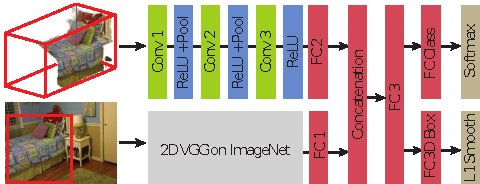
\includegraphics{orn-system-drawing}
    \caption{\textbf{Joint Object Recognition Network:} For each 3D region proposal,
    the 3D volume from depth is fed to a 3D ConvNet and the 2D projection of the
    3D proposal is fed to a 2D ConvNet. Jointly they learn the object category
    and 3D box regression.}
    \label{fig:system}
\end{figure}

The structure of the object recognition network can be seen in figure \ref{fig:system}.
It starts with both a 3D and a 2D object recognition network which are then combined
for the joint recognition.

For the 3D object recognition every proposal bounding box is padded with \(12.5\%\)
of the size in each direction to encode contextual information. The space is divided
into a 30x30x30 voxel grid and TSDF is used to encode the geometric shape of
the object. This network part contains two max pooling layers which use stride 2
and a kernel size of 2x2x2. The three convolution layers use kernel sizes
5x5x5, 3x3x3 and 3x3x3 respectively with a stride of 1 each. Between the fully connected
layers are ReLU and dropout layers (dropout ratio 0.5). The fully connected
layer produces a 4096 dimensional feature vector.

The 2D object recognition part projects the points inside each 3D proposal box
to the 2D image plane. Afterwards the tightest box that contains all these points
is determined. A VGGnet that is pre-trained on ImageNet (without fine-tuning)
is used to extract colour features from the image. The output of VGGnet is then
funneled into a fully connected layer that results in a 4096 dimensional feature
vector.

After both object recognition parts the two feature vectors are concatenated.
Another fully connected layer reduces this feature vector to 1000 dimensions.
These features are used by two separate fully connected layers to predict the
object label and the 3D box surrounding the object.

For every detected box the box size in each direction and the aspect ratio of
each pair of box edges is calculated. These numbers are then compared with a
distribution collected from all the training examples of the same category.
If any of the values falls outside the first to 99th percentile the score
of the box is decreased by \(2\).

The multi-task loss is a sum of classification and regression loss. Cross entropy
is used for the classification loss. The output of the network consists of 20
probabilities (one for each object category). For the regression loss nothing
changes in comparison to the region proposal network. Only difference is the
element-wise normalization of the labels with the object category specific
mean and standard deviation.

After the training of the network concluded the features are extracted from the last
fully connected layer. A Support Vector Machine (SVM) is trained for each object
category. During the testing of the object recognition network a 3D non-maximum
suppression is applied on the results with a threshold of \(0.1\) using the SVM
scores for every box. In case of the box regressions the results from the network
are used directly.

\section{Experimental result and evaluation}

The regional proposal network was trained for 10 hours and the object recognition
network was trained for 17 hours. In both cases an Nvidia K40 GPU was used.
During testing phase it took the RPN \(5.62\) seconds per image and the ORN
\(13.93\) seconds per image. Both networks were evaluated on the NYUv2\cite{Silberman2012}
and SUN RGB-D\cite{Song2015} data sets.
A threshold of \(0.25\) was used to calculate the average recall for the proposal
generation and the average precision for the detection. The SUN RGB-D data set
was used to obtain the ground truth amodal bounding boxes.

\begin{table}
    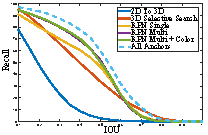
\includegraphics[scale=0.85]{results-drawing-1}
    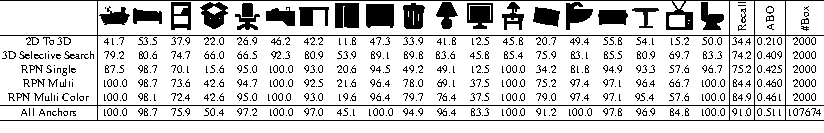
\includegraphics[scale=0.85]{results-table-1}
    \caption{\textbf{Evaluation for Amodal 3D Object Proposal:} [All Anchors] shows
    the performance upper bound when using all anchors.}
    \label{tab:results-object-proposal}
\end{table}

For the evaluation of the proposal generation a single-scale RPN, a multi-scale RPN
and a multi-scale RPN with RGB colour added to the 3D TSDF were compared with
each other and the baselines using the NYU data set. 3D selective search
and a naive 2D to 3D conversion were used as baselines. The naive conversion used the
2D region proposal to retrieve the 3D points within that region. The results can
be seen in table \ref{tab:results-object-proposal}. Afterwards the
outermost 2 percentiles in each direction were removed and a tight 3D bounding
box calculated. The values of recall averaged over all object categories were
\(34.4\) for the naive approach, \(74.2\) for 3D selective search, \(75.2\) for
the single-scale RPN, \(84.4\) for the multi-scale RPN and \(84.9\) for the
multi-scale RPN with added colour. The last value is used as the final region
proposal result.

\begin{table}
    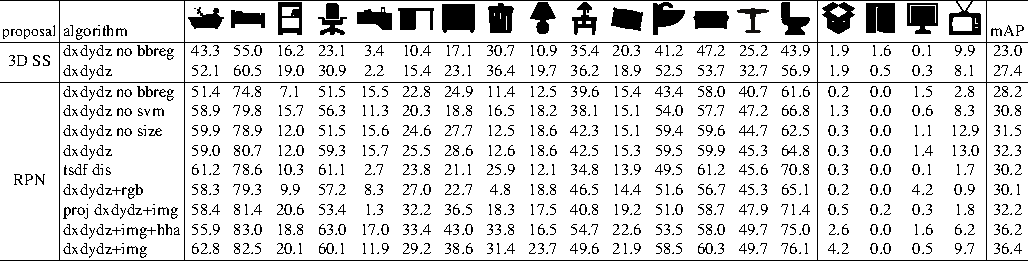
\includegraphics[scale=0.85]{results-table-2}
    \caption{\textbf{Control Experiments on NYUv2 Test Set.} Not working:
    box (too much variance), door (planar), monitor and tv (no depth).}
    \label{tab:results-control-experiments}
\end{table}

Another experiment tested the detection results for the same ORN architecture
given different region proposals (see table \ref{tab:results-control-experiments}).
Comparing the 3D selective search with
RPN gave mean average precisions of \(27.4\) and \(32.3\) respectively. Hence
the RPN provides a better solution. Planar objects (e.g. doors) seem to work
better with 3D selective search. Boxes, monitors and TVs don't work for the RPN,
where the presumed reason for boxes is the high variance and for monitors and TVs
the missing depth information is likely responsible.

The detection evaluation was structured differently. First the feature encodings
were compared with each other (the same experiment that was mentioned in previous
paragraph), then the design was justified and lastly the results were compared
with state-of-the-art methods. The feature encoding experiment provided better
results for encoding the directions directly compared to a single distance.
An accurate TSDF measured better than a projective one. The usage of the 2D image
VGGnet proved to be better than the direct encoding of colour on 3D voxels.
Lastly it didn't help to include HHA (horizontal disparity, height above ground
and the angle the pixel's local surface normal makes with the inferred gravity
direction).

The same experiment was used to help with design choices. It was found that
bounding box regression helps significantly (increase in mAP of 4.4 and 4.1
for 3D selective search and RPN respectively compared to the case without this
regression). SVM was found to outperform the softmax slightly (increase of 0.5 mAP)
which presumably is the case, because it can better handle the unbalanced number of
training samples for each category in the NYUv2 data set. Size pruning was identified
as helping (increase of mAP per category of 0.1 up to 7.8).

\begin{table}
    \centering
    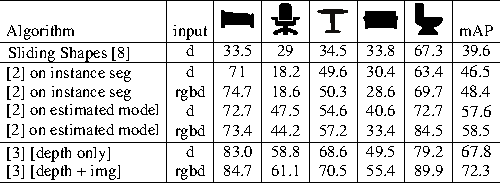
\includegraphics{results-table-3}
    \caption{\textbf{Comparison on 3D Object Detection.}}
    \label{tab:results-object-detection}
\end{table}

For the comparison with state-of-the-art methods Song and Xiao used 3D Sliding
Shapes\cite{Song2014} and 2D Depth-RCNN\cite{Gupta2015} and the same test set
that was used for the 2D Depth-RCNN (intersection of NYUv2 test set and Sliding
Shapes test set for the five categories bed, chair, table, sofa/couch and toilet).
The comparison in table \ref{tab:results-object-detection} shows that 3D Deep
Sliding Shapes outperforms the chosen state-of-the-art methods in all categories.
The toilet is the only example where it is relevant for the result that the 2D
data is used. With only 3D data used the 2D Depth-RCNN performs better on the
estimated model if it uses 2D and 3D.

All in all 3D Deep Sliding Shapes works well on non-planar objects that have depth
information. The 2D component helps in distinguishing similar shaped objects.

\section{Discussion} % (fold)
\label{sec:discussion}

Deep Sliding Shapes offers a seemingly powerful new approach for object detection
in a 3D environment.

\subsection{Paper Strengths} % (fold)
\label{sub:paper_strengths}

The paper is written in a clearly structured way and uses sub headlines to
better guide the reader. The authors apparently tried to minimize repetition
in the sentences and are using some elements of novelized storytelling like
rhetorical questions that soften up the paper and make it less dry. The introduction
in particular is giving a very good motivation for the paper and ends with a cliff
hanger that creates excitement to continue reading beyond the detour that is
the section about related works.

Overall the paper provides many illustrating figures that make it far easier
to imagine the results of the introduced method and quite simply hydrate the
paper and make it friendlier to the eyes compared to an all text paper.

Furthermore the paper provides many evaluation results that are understandable
largely without the main paper text and give a good overview over the performance
of the proposed method compared to others.

Aside from the paper writing skills the authors clearly posess, the presented
approach itself is also very good. It is an elegant idea to first reduce the
search volume by applying a region proposal network and then use an object recognition
network to do the heavy lifting. The usage of the 2D data is well thought of
as well. This abstract idea of dealing with 3D data has persisted and is somewhat
repeated by the Frustum Pointnet\cite{Qi2017}, which uses the results of a 2D
object detection network to determine the region in which the 3D object detection
takes place. The object detection network not only provides the region in form
of bounding boxes but also the classification of the detected objects in form
of a k vector. Though the specific implementation varies greatly the abstract
idea of region proposal, usage of 2D data and object detection/recognition at
the end is visible in both Deep Sliding Shapes and the Frustum Pointnet.

% subsection positive_aspect (end)

\subsection{Paper Weaknesses} % (fold)
\label{sub:paper_weaknesses}

That said there are things to criticize about this paper. The information about
the network structure is spread over two figures and some sections of the paper,
with no guarantees that no information is missing. The evaluation sections are
inconsistent in their structure. The first section about object proposal evaluation
follows the rest of the paper and is written in continuous text. It describes the
compared methods and then discusses the results. However the second section regarding
the object detection evaluation is written completely different. There is no
continuous text and the compared methods are not really described. Instead the
section is largely used to justify the chosen design. If there was an introductory
text explaining their motivations for this kind of evaluation and guiding the reader
through the process it would not even be a problem. However currently there
is no explanation given why the detection evaluation starts with feature encoding
and is followed by design justification.

Furthermore the motivations for the used data sets NYUv2 and SUN RGB-D are
not quite clear. Which data set is used for what purpose and why? The text
mentions in one sentence that the amodal bounding boxes are obtained from
SUN RGB-D without further explanation. It would have been advantageous
if the actual process of this "obtaining" was explained.

Lastly no information regarding the training, validation and testing data split were
available. While this implementation information does not have to be inside the
paper proper it should have been at least inside appendices to make an independent
replication of results possible. Not directly a problem with the paper itself the decision to
implement a software framework from scratch (Marvin framework) rather than using
a proven existing one like Tensorflow makes it more difficult to utilize the
pretrained models which are indeed available and more importantly to adapt Deep
Sliding Shapes to other data sets and problems. To top it all of, the available
Matlab "glue" code is not well documented.

% subsection negitive (end)

% section review (end)

\section{Conclusion}

Deep Sliding Shapes introduces a 3D convolutional network pipeline for
amodal 3D object detection. This pipeline consists of a regional proposal
network and a joint 2D and 3D object recognition network. Experimental
results show that this approach delivers better results than previous
state-of-the-art methods.

The proposed approach introduced an important general structure for networks
working with 3D data and is roughly and on a high-level visible in more recent
network utilizing 3D data as well. In the practical sphere the custom code
framework and the badly documented code makes it very difficult to replicate the
results independently or even adapt Deep Sliding Shapes to other problems.
In short: Good theory, bad practical implementation.

In future work this method should be compared to other 3D centric object detection
approaches like Frustum Point Net\cite{Qi2017}. Especially a structural comparison
with other 3D approaches is interesting to see if there is a best practice structure
emerging for the handling of 3D data.

\newpage
\printbibliography
\addcontentsline{toc}{section}{Bibliography}% Add to the TOC

\end{document}
